\section{Introduzione}
l'ingegneria del software \`e la materia che introduce i \emph{processi di sviluppo software}
che risolvano i problemi della produzione del \sw .

Quindi avere un approccio ingegneristico al problema, applicando metodi quantificabili
che ci permettono di risolvere i problemi classici che attanagliano la produzione.
\\
l'\textbf{IEEE} dice che:
\begin{quote}
    l'Ingegneria del \sw\ \`e l'applicazione di un approccio discipinato, qauntificabile e sistematico allo sviluppo, alla progettazione e alla manutenzione di un \Sw.
\end{quote}
%---------------------------cose un sw-------------------------------------------------------------------------
\subsection{Cos'\`e un \sw}
Secondo l'\textbf{IEEE} un software \`e:

\begin{quote}
    \textit{ Un Software \`e un insieme di \textbf{Programmi}, \textbf{procedure}, \textbf{regole} e ogni tipo di \textbf{documentazione} realtiva al suo funzionamento, di un sistema di eleaborazione dati} 
\end{quote}
Quindi un software non e' solo il codice, ma anche tutte le regole e soprattutto la \emph{documentazione}.
\\
Di particolare importanza \`e la differenza tra \sw\ amatoriale e professionale.
\begin{enumerate}
    \item \sw\ amatoriale: 
        \begin{itemize}
            \item Non sar\`a usato da altre persone
            \item Non dobbiamo soddisfare dei requisiti
            \item Ci sara un solo sviluppatore
        \end{itemize}
    \item \sw\ professionale:
        \begin{itemize}
            \item Sar\`a usato da altre persone
            \item Deve soddisfare dei requisiti di affidabilit\`a e di qualit\`a
            \item Documentazione necessaria
        \end{itemize}
\end{enumerate}
Quindi \`e evidente che il processo di sviluppo di un \sw\ professionale \`e molto pi\`u
complesso. Quindi necessitiamo di metodi rigorosi per regolare questo processo complesso.

Un ulteriore differenza si pu\`o fare sul \emph{Tipo di \sw }:
\begin{enumerate}
    \item \textbf{ \sw\ commerciali:} ad esempio il pacchetto Office, quindi applicazioni
    cos\`i dette ``on the shelf``
    \item \textbf{ \sw\ shareware:} a prova temporale, ad esempio le cosiddette evaluation copy
    \item \textbf{ \sw\ freeware:} gratuito, con o senza codice sorgente. Rimangono i diritti dell'autore
    \item \textbf{ \sw\ public domain:} pubblico senza diritti
\end{enumerate}
Quali sono allora le fasi fondamentali per lo sviluppo di un \sw ?
\begin{enumerate}
    \item \textbf{Specifica:} Definizione dei requisiti e dei vincoli di progettazione (analisi e specifica).
    \item \textbf{Sviluppo:} Progettazione della soluzione e poi l'implementazione in codice.
    \item \textbf{Testing:} Provare il codice in cerca di errori, oppure verificare che i requisti siano soddisfatti(verifica e convalida).
    \item \textbf{Evoluzione:} modifica del software per addattarlo  a nuovi requisti.
\end{enumerate}

%---------------------------CRISI--------------------------------------------------------------------------
\subsection{Il manifesto della Crisi: la nascita del Ing. del \Sw }
Nel 1968, la produzione \sw\ era completamente allo sbando.
La scrittura del codice non era regolamentate, era quasi un processo ``artistico``.
\begin{itemize}
    \item Quasi sempre c'erano incomprensioni tra sviluppatori e cliente.
    \item Si finiva spesso Out Of Budget
    \item Non si consegnava il prodotto, oppure si superavano le scadenze fissate
    \item \Sw\ non di qualit\`a
\end{itemize}
Quindi da queste problematiche, si sente la necessit\`a di un approccio ingegneristico al problema. Nacque allora l'\emph{\textbf{Ing. del \Sw\ }}
%---------------------------COSTI--------------------------------------------------------------------------
\subsection{Il problema dei costi}
Con il passare degli anni, abbiamo notato un incremento enorme del prezzo dei \Sw.
\\
In passato il costo maggiore, era dato dai componenti \textbf{Hardware}, adesso i componenti
costano molto poco a differenza dei \Sw.
\\
Da Dove vengono questi costi?
\\
Questi costi vengono principalmente dalle fasi di \textbf{Sviluppo} e \textbf{Manutenzione}
\begin{figure}[htbp]
    \centering
    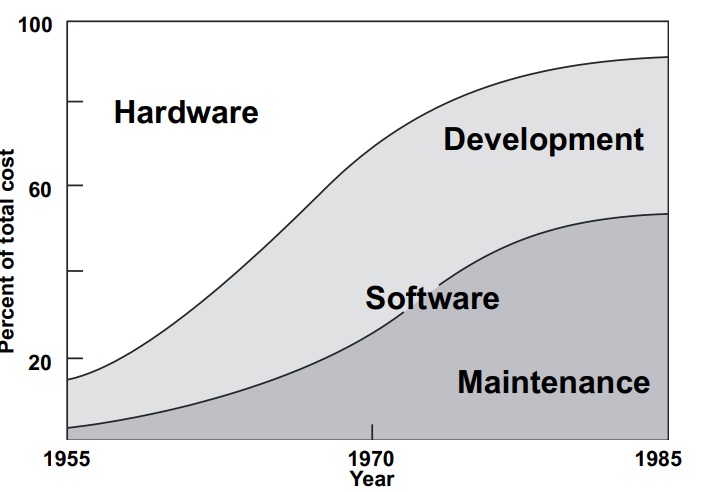
\includegraphics[scale=0.5]{costi.PNG}   
    \caption{Costi negli anni}
    \label{fig:costi}
\end{figure}
\newpage
%---------------------------QUALITA---------------------------------------------------------------
\subsection{Problemi di Qualit\`a}
Vediamo adesso quali sono le caratteristiche di un \sw\ di \textbf{qualit\`a}.
Un \sw\ per essere di qualit\`a deve essere:
\begin{itemize}
    \item \textbf{Manutenibile:} Deve essere facile evolverlo, quindi supportato da una documentazione e codice scritto in maniera pi\`u astratta.
    \item \textbf{Affidabile:} Sebbene sia praticamente impossibile che un \sw\ si privo di errori, la probabilit\`a che avvengano deve rimanere bassa. Caratteristica fondamentale per \Sw\ critici
    \item \textbf{Efficiente:} Deve soddisfare delle richieste in tempi utili(ad esempio i sistemi real-time necessitano tempi precisi e brevi)
    \item \textbf{Accetabile:} Deve essere accettato dagli utenti. Spesso troviamo \sw\ criptici difficilmente comprensibili dagli utenti. Per accetabili inoltre si intendono \sw\ anche che soddisfano le richieste fatte.
\end{itemize}
Spesso queste qualit\`a sono difficili da verificare, in quanto si palesano solo quando il \sw\ viene usato, quindi nella fase operativa.
